\documentclass[11pt]{article}
\usepackage[font=small,labelfont=bf]{caption}
\usepackage{graphicx}
\usepackage{amsmath}
\usepackage{hyperref}\usepackage{color}
\usepackage{parskip}
\usepackage{float}
\usepackage{tabularx}
\usepackage{appendix}
\usepackage{rotating} \usepackage{verbatim} \usepackage{lscape}
\usepackage{dcolumn} \usepackage{ctable} \usepackage{amssymb}
\usepackage{longtable}
\usepackage{threeparttable}
\usepackage{pdflscape}
\usepackage{cases}
 \usepackage[ style=authoryear,backend=biber, url=true]{biblatex}
 \addbibresource{new.bib}

\title{Exporting/Importing and Firm Performance: Evidence from India}
\author{Arjun Gupta}
%\institution{National Institute of Public Finance and Policy}
\newcommand{\alert}[1]{#1}

\newcommand{\floatintro}[1]{
  
  \vspace*{0.1in}
  
  {\footnotesize
    
    #1
    
  }
  
  \vspace*{0.01in}
}
%Introduce floatintros
\definecolor{red}{rgb}{0.0,0.0,0.0}
\hypersetup{colorlinks,breaklinks,linkcolor=red,urlcolor=red,anchorcolor=red,citecolor=red}
\floatstyle{ruled} 
\restylefloat{table} 
\restylefloat{figure}

\begin{document}
\maketitle


\begin{abstract}
 
\end{abstract}


\newpage
\small

\tableofcontents

\newpage

\section{Introduction}\label{sec:introduction}



There is vast literature  which states that exporters/importers tend to
out-perform non-exporters/non-importers  in terms of wages, capital,
productivity. \cite{bernard1999exceptional}  say that this can be due
to these reasons:
\begin{itemize}
\item export/import increases productivity (Self-selection)
\item productivity increases export/import (Learning by doing)
\end{itemize}

Self-selection (SS) hypothesis states that  more productive firms
self-select into export  as  
participation in the trade market is accompanied by additional costs
such as transport costs, establishing a distribution channel,
cost of traversing bureaucratic channels  etc. This means that there
are substantial sunk costs to participating in the trade
market. Therefore, firms which are more productive enter  the
export
market. 

Learning-by-doing hypothesis for exporting (\cite{haidar2012trade}) states that exporting firms deal with
tougher competition in the international market as compared to the
domestic market, and therefore must improve their performance to
remain active in the export market. Moreover, participating in the
international market leads knowledge flows from international buyers
to help post entry performance of export starters. This means that exporting should
cause productivity spillovers as well.

The same hypothesis (self-selection and learning-by-doing) can  apply
to import behavior of firms. Since importing also involves additional
similar costs like additional taxes, transport costs, import duties
etc. , firms that
are more productive will enter the import market. Also, a firm
participating in the import market can have access to higher quality
of intermediated goods. \cite{topalova2011trade}  and \cite{halpern2011imported}
find that improved access to foreign technology can boost
productivity. 

Since  participating in the export/import market   involve sunk
costs, therefore, firms that are the most productive must self-select
themselves into participating in both export and
import market.  Also, it would be interesting to see if participating
in one activity affects participation in the other (i.e
Complementarity between exporting and importing).  I plan to investigate whether there
are benefits of importing to exporting and vice-versa by estimating
the cost complementary nature between the two. 



India provides an interesting case as it liberalised its economy in 1992 which resulted in import
tariffs, deregulation of markets, reduction of taxes, and greater 
foreign investment. According to \cite{topalova2011trade}, \textit{the government's trade policy under the Eighth Five-Year Plan (1992-97) ushered
in radical changes to the trade regime by sharply reducing the role of
the import and export control system. The share of products subject to quantitative restrictions
decreased from 87 percent in 1987‐88 to 45 percent in 1994-95, and the actual user
condition on imports was discontinued. And since 1997, the decrease in
output and input tariff has been very marginal.}

So, my reasearch plan is to investigate:
\begin{itemize}
\item Self-selection hypothesis: Check whether more productive firms
  participate in the expprt/import market
\item Learning-by-doing hypothesis: Check if there are productivity
  spillovers from participation in the export/import market
\item Estimate the fixed and sunk costs of participation in the
  export/import market and the decrease in costs due to the
  complimentary (simultaneous and lagged) nature between the two
\item Run counter-factual experiment to see the effect of decrease in
  the costs to exporting/importing. 
\end{itemize}

\section{Literature Review}
Most papers on this can be differentiated into three different
categories:
\begin{enumerate}
\item Importing and Productivity 
\item Exporting and Producitivity
\item Complimentarity between exporting and importing and its effect
  on productivity
\end{enumerate}
In this section, I write down the major literature contributions
towards my topic. 
\subsection{Importing and Productivity}
\cite{halpern2011imported} studies effect of imports on productivity by estimating a structural
model of importers in a panel of Hungarian firms. They find that imports have
a significant and large effect on firm productivity, about one-half of which is due
to imperfect substitution between foreign and domestic goods. 

\cite{topalova2011trade} find that the procompetitive
effects of the tariffs led firms to become more
efficient, the larger impact appears to have come from 
increased access to foreign inputs.
\subsection{Exporting and Productivity}
\cite{aw2011}  estimate a dynamic structural model that captures both the behavioral
and technological linkages among R\&D, exporting, and
productivity. They find that Relative to a
plant that does neither activity, export market participation raises future productivity
by 1.96 percent, R\&D investment raises it by 4.79 percent, and undertaking both
activities raises it by 5.56 percent. 

 \cite{bernard1999exceptional} test the self-selection and
 learning-by-doing hypothesis of exports on firms. They find that Good
 plants become exporters i.e. learn to export. and find that exporting
 increases the survival probability but it does not contribute towards
 productivity growth.  

\cite{roberts1997decision} quantify the effect of prior exporting
decision on the current exporting decision and test the sunk cost
hypothesis of these activities.  They  develop a dynamic discrete-
 choice model of exporting behavior that separates the roles of profit heterogeneity
 and sunk entry costs in explaining plants' exporting status and find
 that sunk costs are significant as prior export experience increases
 the probability of exporting by 60 percent.  


In terms of work in this field with Indian firm level  data,
\cite{haidar2012trade} and \cite{gupta2018exporting} find evidence of
self-selection of more productive firms into exporting, but they do
not find evidence of learning-by-exporting.  
\subsection{Cost Complementarity between Exporting and Importing}
As far as I am aware, there have been two major papers in this field
i.e \cite{aristei2013firms} and \cite{kasahara2013productivity}. 

\cite{aristei2013firms} estimate a bivariate probit model to
understand the two-way relationship between exporting and importing. 
Thy suse  firm-level data for a group of 27 Eastern European and 
Central Asian countries from the World Bank Business Environment 
and Enterprise Performance Survey (BEEPS) over the period 2002–2008, 
and after controlling for size (and other firm-level characteristics),
find that firms’ exporting activity does not increase the
probability of importing, while the latter has a positive effect
 on foreign sales. 

\cite{kasahara2013productivity} estimate a stochastic model of
exporting and importing that incorporates heterogeneity in transport
costs and estimate export and import complimentarities between the two
trade activities. They find that policies which inhibit the
importation of  foreign intermediates can have a large adverse 
effect on the exportation of final goods.  

\subsection{Productivity Estimation}
Productivity estimation in all of the papers mentioned is done using
the methods highlighted in the papers below:
\cite{olley1992dynamics},\cite{levinsohn2003estimating},
\cite{ackerberg2006structural} and \cite{wooldridge2009estimating}. 
These papers take inspiration from one another and the difference in
estimation mentioned in these papers is very minimal. These methods
have been explained in section \ref{prodest}

Here, \cite{de2013detecting} highlights the importance of endogenising
the export decision in the minimisation problem of the productivity
estimation. 

\section{Data}\label{sec:data}
I use annual firm level data from Centre for Monitoring Indian Economy
(CMIE) which provides  data from 1989 to 2017. 

I fetch the following variables from CMIE: 

\begin{center}
\input{./TABLES/indicatordescription.gen}
\end{center}

Table \ref{indicator} shows the variables and their meaning. I chose the variables
which might be the most pertinent to my research question. 
The variables stated above are nominal values. I fetch Wholseale Price
Index (WPI), which provides the inflation rate of the wholesale prices
and deflate the variables to give real values. Then, I clean the data
to remove missing values and select firms with the broad industry
classification code indicating that they are a manufacturing
firms. Table \ref{compnfirms} shows the composition of firms by year: 
\begin{center}
\input{./TABLES/compnfirms.gen}
\end{center}
 I restrict the time period of the study from 1997 to 2016.  Since, firms
are under no legal obligation to report their finances, which might
mean that mean that small firms are less likely to report their
finances. However, this dataset includes all publicly listed firms as
their firm financials are public information. This might affect my
results as it is biased towards bigger firms. 

I create two additional variables \textit{Export} , \textit{Import},
\textit{Domestic Sales}
by adding the following variables from the Table 1.  
\begin{enumerate}
\item Export: sa\_export\_goods $+$ sa\_export\_serv
\item Import: sa\_import\_rawmat $+$        sa\_import\_stores\_spares
  $+$ sa\_import\_fg            $+$sa\_import\_cap\_goods
\item Domestic Sales: Total Sales - Export Sales
\end{enumerate}
Then, I create four dummy variables of trade market participation
using the \textit{Export} and \textit{Import} variables: 
\begin{itemize}
\item None: Firms that do not participate in the export/import market
\item Export only: Firms that participate in the export market only
\item Import only: Firms that participate in the import market only
\item Both: Firms that participate in both export/import market
\end{itemize}
Table \ref{comp_table} displays the composition of firms according to their trade market
participation status. It is seen that number of firms that do not
participate in the trade market is low,  around 20 to 35
\%. Surprisingly, the number of firms that participate in the trade
market is really high. Another interesting feature is that the number
of firms that participate only in the import market is higher than the
firms that participate only in the export market. This must mean that
the demand for foreign intermediaries is really high. Almost 50 \% of
firms in each year participate in both export/import market.  It is
also seen that the participation rate in the trade is not increasing
year on year.  
\begin{center}
\input{./TABLES/composition.gen}
\end{center}
\section{Descriptive Statistics}
\subsection{Self-Selection}
As a first step to see if more productive firms self-select into
participating in the trade market, I calculate the mean and standard
deviation and created the density plots for log of  sales, gross fixed assets,
salaries and  expenditure on power and fuel for firms with different
trade activity status. 
Tables \ref{lsales}, \ref{lgfa}, \ref{tab:lsalary} and \ref{tab:lrawmat} the results for the variables mentioned above. 
It can be seen that firms that participate in the trade market have
higher mean for all the variables mentioned above. It is also seen
that firms that participate in the both export/import market have
higher mean of sales,gross fixed assets,
salaries, expenditure on power and fuel than firms that participate in
only export and only import. On the other hand, the standard deviation in all
the cases is very similar. This indicates that firms participating
in the trade market has an positive effect on the characteristics of the firm.
\begin{center}
\begin{table}[htp]
\caption{Summary statistics of Sales (log)}
\label{lsales}
\begin{tabular}{c}
 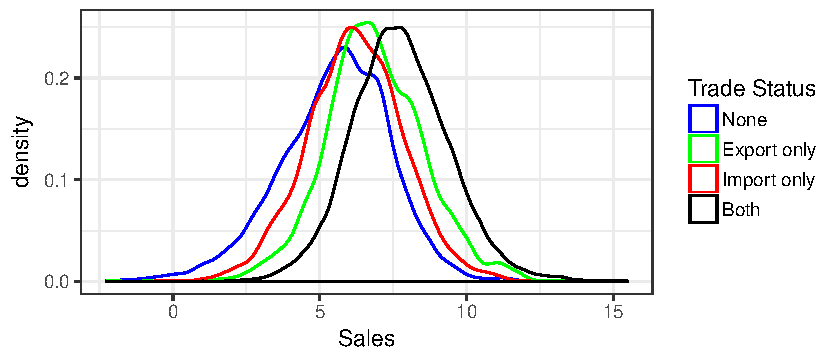
\includegraphics{./PICS/denslsales.pdf}   \\ 
 \input{./TABLES/sumstatslsales.gen}  \\  
\end{tabular}
\end{table}
\end{center}
\begin{center}
\begin{table}[htp]
\caption{Summary statistics of Gross Fixed Assets (log)}
\label{lgfa}
\begin{tabular}{c}
 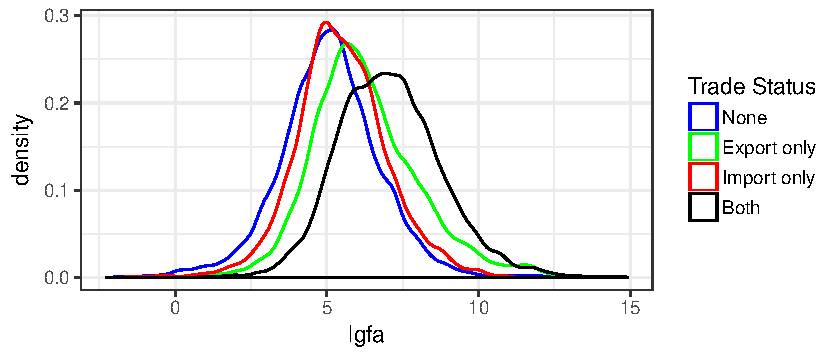
\includegraphics{./PICS/denslgfa.pdf}   \\ 
 \input{./TABLES/sumstatslgfa.gen}  \\  
\end{tabular}
\end{table}
\end{center}
\begin{center}
\begin{table}[htp]
\caption{Summary statistics of Salary (log)}
\label{tab:lsalary}
\begin{tabular}{c}
 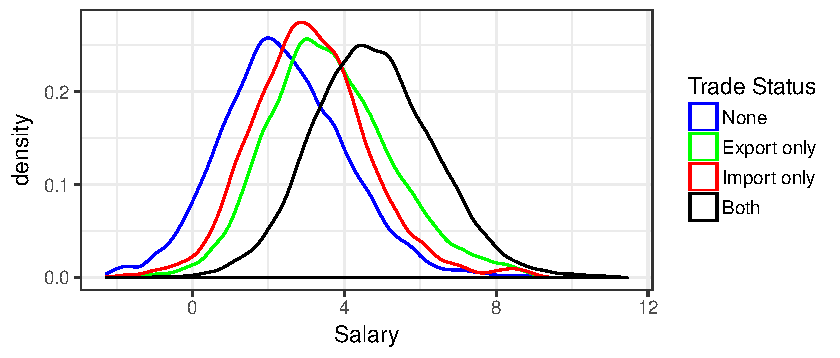
\includegraphics{./PICS/denslsalary.pdf}   \\ 
 \input{./TABLES/sumstatslsalary.gen}  \\  
\end{tabular}
\end{table}
\end{center}
\begin{center}
\begin{table}[htp]
\caption{Summary statistics of Expenditure on raw material (log)}
\label{tab:lrawmat}
\begin{tabular}{c}
 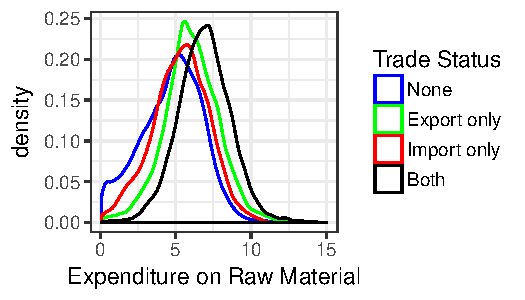
\includegraphics{./PICS/denslrawmat.pdf}   \\ 
 \input{./TABLES/sumstatslrawmat.gen}  \\  
\end{tabular}
\end{table}
\end{center}
\subsection{Trade Premia}
Trade premia is defined as the difference in
attributes of firms based on their trade participation status. I
estimate the trade premia using the following regression:
$$ X_{it} = \alpha + \beta_{1} d_{it}^{X}+ \beta_{2} d_{it}^{M}+
\beta_{3} d_{it}^{X}*d_{it}^{M} + \beta_{4} age_{it} + \epsilon_{it}$$
where $X_{it}$ is firm level characteristics such as Sales, Gross
Fixed Assets, Expenditure on Raw Material and Salary, $d_{it}^X$ is
the export dummy,$d_{it}^M$ is
the import  dummy, the interaction term between these two variables
and $age_{it}$ is the age of the firm. I estimate this equation using
fixed-effects regression controlling firm and time fixed
effects. Table \ref{expimppremia} displays the results for the above
regression. 
\begin{center}
\input{./TABLES/expimppremia.gen}
\end{center}
It is seen coefficients for both export and import dummy are positive
and significant at 1\% significance level. This means that firms that
participate in the export/import market have more capital and assets
and spend more on salary and raw materials than firms that do not
participate in the trade market. The interaction term between the
export and import dummy is very low in two cases and not significant
in the other two. This means that firms that participate in the both
export and import have  higher sales,assets etc. than firms that
participate in one of these trade activities. The age variable also
has a positive coefficient and is significant at 1\% significance
level. Therefore, the older a firm becomes the higher its capital,
assets etc. become. 

\subsection{Complementarity between Exporting and Importing}
Table \ref{tab:lexport} displays the export value for firms that participate only in the
export market and for firms that participate in both export/import
market. 
It is seen in Table \ref{tab:lexport} that firms that participate in both the
export/import market have a higher exports than firms that only
participate in the export market. This suggests that importing has a
positive effect on exporting.   
\begin{center}
\begin{table}[htp]
\caption{Summary statistics of Export (log)}
\label{tab:lexport}
\begin{tabular}{c}
 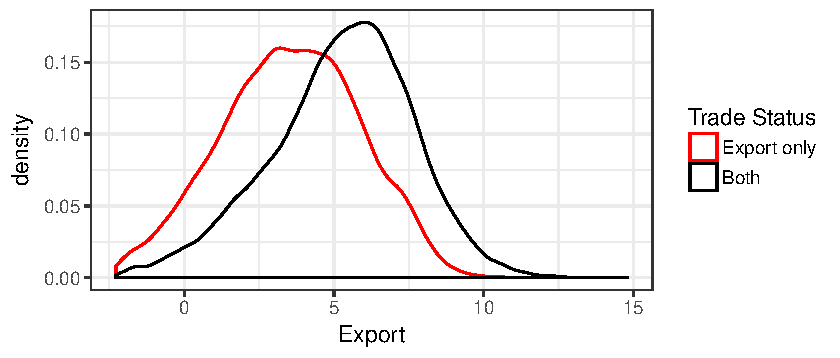
\includegraphics{./PICS/denslexport.pdf}   \\ 
 \input{./TABLES/sumstatslexport.gen}  \\  
\end{tabular}
\end{table}
\end{center}
Table \ref{tab:limport} displays the import value for firms that participate only in the
import market and for firms that participate in both export/import
market. 
It is seen in Table \ref{tab:limport} that firms that participate in both the
export/import market have a higher imports than firms that only
participate in the import market. This suggests that exporting has a
positive effect on importing.  

\begin{center}
\begin{table}[htp]
\caption{Summary statistics of Import (log)}
\label{tab:limport}
\begin{tabular}{c}
 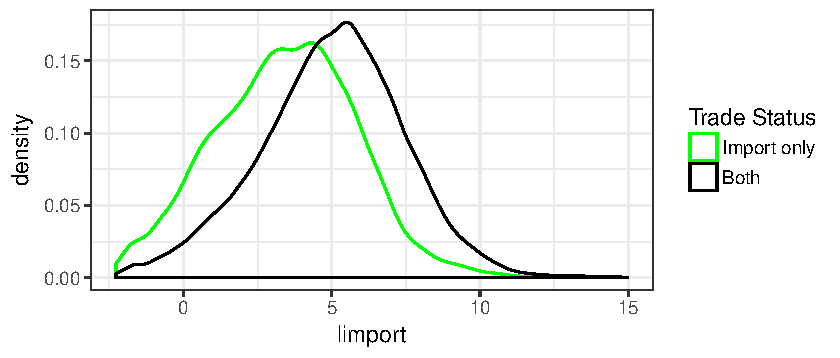
\includegraphics{./PICS/denslimport.pdf}   \\ 
 \input{./TABLES/sumstatslimport.gen}  \\  
\end{tabular}
\end{table}
\end{center}
Tables \ref{tab:lexport}and   \ref{tab:limport} suggest that both these activities have a
positive effect on the other and this might be because importing
complements exporting and vice-versa. Therefore, there is correlation between these
activities that needs further research. 

The first two columns of table \ref{prodpremia} estimates the
following regressions:

$$  ln(Export)_{it} = \alpha +  \beta_{1} d_{it}^{M}+
+ \beta_{2} age_{it} + \epsilon_{it}$$

$$  ln(Import)_{it} = \alpha + \beta_{1} d_{it}^{X} + \beta_{2} age_{it} + \epsilon_{it}$$ 

\begin{center}
\input{./TABLES/prodpremia.gen}
\end{center}

It is seen that the discrete decision to import has a positive and
significant effect on the value of imports. The discrete decision to
export also has a positive and significant effect on the quantity of
imports.  This further suggests the evidence of complimentarity
between exporting and importing. 
\subsection{Productivity and Export/Import}
\cite{gupta2018exporting} define a rough measure of productivity known
as \textit{capital productivity}. It is defined as the log of value added per
unit of capital used by a firm:

$$ log(VA_{it} - log(K_{it}))$$
where $VA_{it}$ is firm-level value added, computed as total industrial sales plus
change in stock minus power and fuel expenditures, and raw material
expenses. Table * displays the summary statistics for this variable
based on the trade activity status. It can be seen that mean of capital
productivity increases as activity status moves from \textit{None} to
\textit{Export only/Import only} to \textit{Both}, whereas the
standard deviation also decreases.  
\begin{center}
\begin{table}[htp]
\caption{Summary statistics of Capital Productivity (log)}
\label{tab:capprod}
\begin{tabular}{c}
 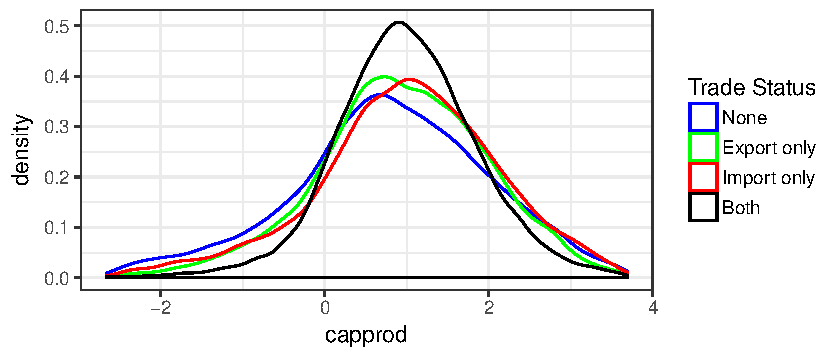
\includegraphics{./PICS/denscapprod.pdf}   \\ 
 \input{./TABLES/sumstatscapprod.gen}  \\  
\end{tabular}
\end{table}
\end{center}

Table \ref{tab:capprod} displays the summary statistics of Profit to Sales based on a
firms trade market status. Profit to sales is calculated by dividing
the profit after tax with sales. This measure can be interpreted as a
profitability measure. It is seen in table \ref{tab:capprod} that participating in
the trade market increases the profit to sales ratio. Firms that do
not participate in the trade market have a very high standard
deviation of profit to sales. It is also interesting to see that mean
profit to sales ratio in every case is negative. 
\begin{center}
\begin{table}[htp]
\caption{Summary statistics of Profit to Sales}
\begin{tabular}{c}
 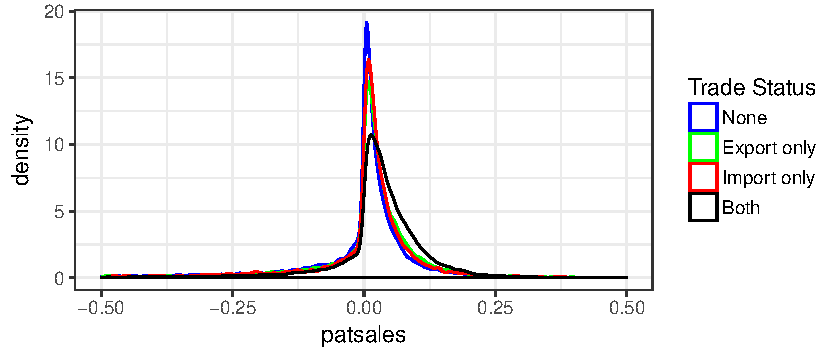
\includegraphics{./PICS/denspatsales.pdf}   \\ 
 \input{./TABLES/sumstatspatsales.gen}  \\  
\end{tabular}
\end{table}
\end{center}
 
The last two columns of table \ref{prodrpemia} estimate the trade
premia for the crude measures of the productivity defined above i.e
Capital Productivity and Profit-to-sales ratio. It is seen that both
of the crude measures of productivity react positively to the discrete
decisions to import and export. Moreover, since the interaction term
is not significant, this means that participation in both activities
leads to higher productivity than participation in one activity. 
\subsection{Transition Probability}
Table \ref{tab:transition} displays the transition probabilities observed in the data. It
can be seen that there are very high levels of persistence from
\textit{None} in t-1 to \textit{None} in t  and from \textit{Both} in
t-1 to \textit{Both} in t. This means that there must be high fixed
costs to enter in the export/import market since only 12\% of the
firms  that do not participate in the trade market in t-1 start
participating in the trade market in t. The high levels of persistence
in \textit{Both} must mean that this mechanism benefits the firms in a
lot of ways. The levels of persistence in \textit{Import Only} and \textit{Export Only}  is not as high. A large
portion of firms switch to participating in both the trade market
activities.This can mean that participating in the export in time
period in t-1 complements participating in the export market in period
t and vice-versa. Also, the number of firms that flip-flop (i.e switch
trade market status) is low, this can mean that there are fixed costs
to participating in the stock market as well. 
\begin{center}
\begin{table}[!htp]
\caption{Transition probability}
\label{tab:transition}
\input{./TABLES/transition.gen}
\end{table}
\end{center}

\section{Preliminary Analysis}
Before modelling this behavior, I try to check if the phenemenon
mentioned above are seen in the data. 

I divide this into three parts and check whether: 
\begin{itemize}
\item Learning-by-doing: How does lagged choice of export/import
  impact productivity?
\item Self-Selection: Selection of more productive firms into
  exporting/importing
\item Complementarity between exporting and importing: Does engaging
  in one activity complements participation in the other?
\end{itemize}
\subsection{Learning-by-doing}
I use \cite{levinsohn2003estimating} to estimate productivity using  a Cobb-Douglus production function: 
\begin{equation}
y_{it} = \beta_{o} + \beta_{l}l_{it} + \beta_{k}K_{it} +
\omega_{it}(m_{it}, k_{it}) + \eta_{it} 
\end{equation}
I use the variable gross fixed assets as a measure of capital, salary
as a measure of labor and a expenditure on raw materials as a measure
of intermediated input. The estimation procedure has been described
below (see here \ref{lp}). Since \cite{levinsohn2003estimating} assume
a markovian nature of productivity evolution, where the
productivity evolution is assumed to follow the procedure below:
$$ \omega_{it} = \alpha_{o} + \alpha_{1}\omega_{it-1} +
\alpha_{2}\omega_{it-1} + \alpha_{3}\omega_{it-1}^{2}+
\alpha_{4}d_{it-1}^{X} + \alpha_{5} d_{it-1}^{M} +
\alpha_{6}d_{it-1}^{X}d_{it-1}^{M}  + \nu_{it}
$$ 
where $d_{it-1}^{X}$ and $d_{it-1}^{M}$ is the discrete decision to
export and import respectively. 
 I use the method highlighted in \cite{de2013detecting}  to accommodate endogenous
productivity evolution which allows  past export experience to impact
the evolution of capital. The estimates of the productivity evolution
are shown in Table \ref{prod}. The Cobb-Douglus coefficients are shown in
Table \ref{regLP}. 
\input{./TABLES/regLP.gen}
\input{./TABLES/prod.gen} 

\cite{de2013detecting} say that exogenously accomodating the
decision to export/import mplies that
past export/import experience has no impact on direct technological
improvements. Therefore, the coefficient of capital will be biased if
the trade market decisions is correlated with capital. Table
\ref{regLPex} displays the coefficients when the export/import
decision is not endogenously allowed to contribute towards the
productivity evolution. In this case, the coefficient of capital is
biases upwards since the variation in output is attributed more
towards capital.   
\input{./TABLES/regLPex.gen}

Table \ref{regLPcont} and \ref{prodcont} display the Cobb-Douglus coefficients when the
productivity is dependent on the continuous value of export and import
and they show results similar to the ones shown in tables \ref{regLP} and \ref{prod}. 
It is seen that productivity evolutions depends non linearly on past
productivity. The interesting result is that lagged exporting does not a have
a significant effect on productivity. However, it is seen that
importing does have a significant effect on productivity i.e the
decision to import causes the productivity to increase by 3 per
cent. The interaction term between exporting and importing also does
not have a significant effect on productivity. Based on these results, I
conclude that manufacturing firms experience learning-by-importing and
do not experience learning-by-exporting.

In the next section, I check whether more productive self-select into
exporting/importing 
\subsection{Self-Selection}
I use the following equations  to verify that more productive firms
self-select into participating in the export/import market:
\begin{equation}
\hat{log(TFP)_{t-j}} = \gamma_{1}log(export)_{it}+ \gamma_{2}log(import)_{it} +
 \beta c_{i,t-j}
\end{equation}

\begin{equation}
\hat{log(TFP)_{t-j}} = \gamma_{1}d_{it}^{X}+ \gamma_{2}d_{it}^{M} +
\gamma_{3}d_{it}^{X}d_{it}^{M} + \beta c_{i,t-j}
\end{equation}
where $c_{i,t-j}$ contains log of capital and labour. I estimate the
equation mentioned above for three time periods $j=1,2 \& 3$ and for
the discrete decision as well as the value of exports/imports.  The
coefficients are estimated using fixed-effects regression. 
Table \ref{discprod} and Table \ref{contprod} display  $\gamma$ estimates for equation 2 and 3
respectively
  
\input{./TABLES/discprod.gen}
\input{./TABLES/contprod.gen}
In the discrete case, productivity of firms which export in year t is
12.5 \%, 7\% and 4.2 \% higher than non-exporting firms in in year
t-1,t-2 and t-3 respectively. And the productivity of firms which
import in year t is 13.8 \%, 8\% and 4.9 \% higher than non-nonimporting firms in in year
t-1,t-2 and t-3 respectively. The interaction variables are
not significant in all the three cases. This suggests that for firms
to participate in both the markets, their lagged productivity needs to
be higher than firm who participate in either the export or the export
market. Another interesting feature is that firms that only import in
year t have higher lagged productivity than firms that only export in
year t.

Tables\ref{discprod} and  \ref{contprod} provide evidence that lagged productivity at for all the three
time periods before is higher when the firm participates in the export
market in year t. This gives evidence of self-selection of firms into
exporting and importing as the lagged productivity for three
consecutive time periods before exporting/importing has a
significantly positive value. 
\subsection{Complimentarity between exporting and importing}
According to \cite{roberts1997decision}, the Bellman equation for an
exporting market participation can be decomposed into dynamic discrete
choice model. Since this study takes both exporting and importing into
account, the export and import decision is modelled as a bivariate dynamic
probit  with the discrete decision of exporting and importing as
dependent variables.  

Let $d_{it}^{X}$ be the discrete decision to participate in export
market and $d_{it}^{XM}$ be the discrete decision to participate in import
market.  Then, the bivariate dynamic probit model takes the following form 

\begin{equation}
  d_{it}^{X}=\begin{cases}
   1 , & \text{if $d_{it}^{X*}>  0$}.\\
   0 , & \text{if $d_{it}^{X*}<  0$}.
  \end{cases}
\end{equation}

\begin{equation}
  d_{it}^{M}=\begin{cases}
   1 , & \text{if $d_{it}^{M*}>  0$}.\\
   0 , & \text{if $d_{it}^{M*}<  0$}.
  \end{cases}
\end{equation}
The discrete decision of exporting and importing is modelled as a function of previous import and
export status controlling for lagged firm characteristics and industry and time fixed
effects. 
\begin{equation}
d_{it}^{X*} = \gamma_{1}^{X} d_{it-1}^{X} + \gamma_{2}^{X} d_{it-1}^{M}+
\gamma_{3}^{X} \hat{\omega}_{it-1}  + \beta_{1}^{X}K_{it-1}  +
IndustrialDummy_{i}^{X} + TimeDummy_{t}^{X}  + \epsilon_{it}^{X}
\end{equation}
Here $\gamma_{1}$ identifies the state dependence coefficient, $\gamma_{2}$ accounts for
the fact that participating in one activity in time t-1 improves the
odds of participating in the other at time t,$\gamma_{3}$ accounts for
the self-selection mechanism, $\beta_{1}$ accounts for capital at time
t-1 and $IndustrialDummy_{i}^{M}$  $TimeDummy_{t}^{M}$ are industrial
and time dummies respectively.
\begin{equation}
d_{it}^{M*} = \gamma_{1}^{M} d_{it-1}^{M} + \gamma_{2}^{M} d_{it-1}^{X}+
\gamma_{3}^{M} \hat{\omega}_{it-1}  + \beta_{1}^{M}K_{it-1}  +
IndustrialDummy_{i}^{M} + TimeDummy_{t}^{M}  + \epsilon_{it}^{M}
\end{equation}

The bivariate specification also allows for the
contemporaneous correlation between the two choices as
$\epsilon_{it}^{X}$ and $\epsilon_{it}^{M}$ are allowed to be
correlated. This gives gives the following form to the error
structure: 


\[\begin{pmatrix}
\epsilon_{it}^{X} \\
\epsilon_{it}^{M}
\end{pmatrix}\sim N\left(\begin{pmatrix}
0 \\
0
\end{pmatrix},\begin{pmatrix}
1 & \rho \\
\rho & 1
\end{pmatrix}\right)
\]
This model specification has been used to test the contemporaneous relationship
by \cite{aristei2013firms} and \cite{aw2011}. 
The initial conditions problems is treating by assuming that $d_{i1}$ is 
endogenously given. The  equation is estimated by assuming that lagged
firm characteristics and industry and time  dummy variables account
for the differences between firms, negating the use of a random
effects model. 
\begin{center}
\begin{table}[htbp]
\caption{Dynamic Probit Estimates}
\begin{tabular}{@{\extracolsep{5pt}}lcc} 
\\[-1.8ex]\hline 
\hline \\[-1.8ex] 
 & \multicolumn{2}{c}{\textit{Dependent variable:}} \\ 
 & $d_{it}^{X}$ & $d_{it}^{M}$ \\
\cline{2-3} 

$d_{it-1}^{X}$ & 2.520*** & 0.407*** \\
 & -158.98 & -25.13 \\
$d_{it-1}^{M}$ & 0.388*** & 2.173*** \\
 & -21.58 & -136.24 \\
$\hat{\omega_{it-1}}$ & 0.0759*** & 0.126*** \\
 & -8.97 & -15.72 \\
$K_{it-1}$ & 0.0220** & 0.0899*** \\
 & -2.88 & -12.23 \\
$L_{it-1}$ & 0.107*** & 0.106*** \\
 & -13.62 & -13.92 \\
cons & -2.068*** & 0.446*** \\
 & (-14.17) & -31.66 \\
$\rho$ & 0.4457163*** &  \\
 & (-0.01407) &  \\
N & 67593 &  \\
\hline 
\hline \\[-1.8ex] 
\textit{Note:}  & \multicolumn{2}{r}{$^{*}$p$<$0.1; $^{**}$p$<$0.05; $^{***}$p$<$0.01} \\ 
\end{tabular}
\end{table}
\end{center}
Table 13 displays the results for dynamic probit specification. All
  the coefficients are significant at 1\% level.  The
  state-dependence coefficient has the strongest effect amongst all
  the variables, suggesting that there is persistence in both the
  activities. There is a positive effect of lagged
  productivity on both activities, providing further evidence of
  self-selection of firms into exporting and importing. 

The results suggest a two-way relationship between exporters and
  importers: Firms which were importing in the previous year are more
  likely to be exporters and firms which were exporting in the
  previous year are more likely to be importing this year. Also, the
  correlation between the errors represented by $\rho$ is
  significantly different than zero suggesting that there simultaneous
  complementarity between exporting and importing.
\subsection{Conclusion}

The results from this section and descriptive statistics suggest a few
overall themes of the data: 
\begin{itemize}
\item Learning-by-doing: I estimate productivity using
  \cite{levinsohn2003estimating} such that they are dependent on the
  lagged export and import choices and I get the following results for
  the two trading activities:
\begin{enumerate}
\item Export: Firms do not display learning-by-exporting as the
  coefficient of discrete choice of lagged export decision does not
  have a significant effect on productivity. 
\item Import: Firms display learning-by-exporting a the
  coefficient of discrete choice of lagged import decision does
  have a significant effect on productivity 
\end{enumerate}
\item Self-Selection: I regress the lagged productivity values of the
  estimated productivity for $t= t-1,t-2$ and $t-3$ on the discrete choice
  of exporting and importing after controlling for firm
  characteristics and industry and time fixed effects and get the
  following result:
\begin{enumerate}
\item Export: The coefficient for the discrete export choice has a
  positive effect significant at 1\% level on the lagged values of
  productivity. This suggests that firms learn to export.  
\item Import:  The coefficient for the discrete import choice also has a
  positive effect significant at 1\% level on the lagged values of
  productivity. This suggests that firms learn to import as well. 
\end{enumerate} 
\item Complementarity between exporting and importing: I run a
  bivariate dynamic probit regression of discrete choice of
  exporting/importing on their lagged values, firm characteristics and
  industry and time dummies to get the following results:
\begin{enumerate}
\item Export: There is strong persistence in exporting behavior,
  lagged import decision has a positive effect on current exporting
  behavior. 
\item Import: There is strong persistence in importing behavior,
  lagged export decision has a positive effect on current importing
  behavior. 
\item: Simultaneous Complementarity: There is a strong presence of
  simultaneous complementarity since the errors for the equations are
  highly correlated are significant at 1\% level.  
\end{enumerate}
The bivaraite dynamic provide  results suggest that there is strong cost complementarity
between exporting at time t with importing at time t and t-1 and
vice-versa. But, the learning by export result show that there is no
learning by exporting. This must mean that importing must help in
reducing the cost to export since they do not enter the productivity
mechanism. 

\end{itemize}

\section{Model}

I use a model inspired from  \cite{aw2011}, \cite{de2011product} and \cite{kasahara2013productivity}. 

\subsection{Static Decision}

A firm i has a standard Cobb-Douglas Production Function 

\begin{equation}
Q_{it} =
k_{it}^{\alpha_k}L_{it}^{\alpha_l}M_{it}^{\alpha_m}exp(\omega_{it} + u_{it})
\end{equation}
where 
\begin{itemize}
\item $K_{it}$ is the unit of output
\item $L_{it}$ is the unit labour
\item $M_{it}$ is the domestic and imported unit of materials
\item $\omega_{it}$ is the productivity shock
\item $u_{it}$ is the measurement error
\end{itemize}

A firm faces a constant elasticity of demand (CES) function assumed to
be of the Dixit-Stiglitz form :

\begin{equation}
Q_{it}^{D} = Q_{dt}(\frac{P_{it}}{P_{dt}})^{\eta_{d}}
\end{equation} 
where $Q_{idt}^{d}$ is the industry aggregate output, $P_{dt}^{d}$ is
the price index and $P_{it}^{d}$ is the firm i's price. 

The demand function in the export market has a similar structure
except that it also depends on an industry-specific demand shifter: 
\begin{equation}
Q_{it}^{X} = Q_{Xt}(\frac{P_{it}^{X}}{P_{dt}^{X}})^{\eta_{X}}exp(z_{it})
\end{equation} 
where $z_{it}$ is the unobserved firm specific demand
shock. 

Equation 2 can be used to obtain an expression for $P_{it}$ and a
firms domestic revenue is $R_{it} = P_{it}Q_{it}$, and inserting price
into the revenue function and taking a log to get the revenue function
in the domestic market:

\begin{equation}
\tilde{r_{it}} = \beta_{l}l_{it} + \beta_{m}M_{it} + \beta_{K}K_{it} +
\beta_{d}Q_{dt} + \omega^{*}_{it} + u_{it}
\end{equation}
 The revenue function for the export market can be similarly derived
 to get:
\begin{equation}
\tilde{r_{it}} = \beta_{l}l_{it} + \beta_{m}M_{it} + \beta_{K}K_{it} +
\beta_{X}Q_{Xt} + \omega^{*}_{it} + u_{it} + z^{*}_{it}
\end{equation}
where $\beta_{h}= \frac{\eta_{d}+1}{\eta_{d}}\alpha_{h}$, $\beta_{s.m} =
\frac{1}{\eta_{d}}$, $\omega^{*}_{it} =
\omega^{*}_{it}\frac{\eta_{d}+1}{\eta_{d}}$ and $z^{*}_{it} =
z_{it} eta_{d}^{-1}$


\cite{das2007market} display a relation between profits and revenue. I
use this estimate the constant demand of elasticity in both the
domestic and export market. 
In the domestic market, the profits are: 
\begin{equation}
\pi_{it}^d = \frac{1}{\eta_{d}} r_{it}^{d}(K_{it}, \omega_{it})
\end{equation} 

In the export market, the profits are: 
\begin{equation}
\pi_{it}^X = \frac{1}{\eta_{X}} r_{it}^{X}(K_{it}, \omega_{it})
\end{equation} 

\subsection{Transition of Productivity}

The firm-level productivity is allowed to the be endogenously affected
by the firms decision to export and import. Therefore, the law of
motion of productivity is:

\begin{equation}
\omega_{it} = g(\omega_{it-1}, d_{it-1}^{X}, d_{it-1}^{M}) + \nu_{it}
\end{equation}

\begin{equation}
\omega_{it} = \alpha_{o} + \alpha_{1}\omega_{it-1} +
\alpha_{2}\omega_{it-1} + \alpha_{3}\omega_{it-1}^{2}+
\alpha_{4}d_{it-1}^{X} + \alpha_{5} d_{it-1}^{M} + \alpha_{6}d_{it-1}^{X}d_{it-1}^{M}  \nu_{it}
\end{equation}

where $d_{it-1}^{X}$ is an indicator function of the firms lagged export
participation, $d_{it-1}^{M}$ is an indicator function of the firms lagged import
participation and $\nu_{it}$ is an iid shock to the productivity. The
lagged export and import indicator variables allow for
learning-by-exporting and productivity benefits from importing. 

The model assumes that productivity is only affected by the intensity
of export/importing but is only dependent on the decision. 

The firm-specific demand shock is modelled as an AR(1) process. 


\subsection{Dynamic Model}
 
Firm must pay a fixed/sunk costs of trading. Let $d_{i,t}^X$ be the
indicator function of participation in the export market and
$d_{i,t}^M$ be the indicator function of participation in the import
market. Then the total costs paid by firm i in period t is given by:


$F(d_{it}, d_{it-1})= $
\begin{enumerate}
\item   $f^{x} + c^{X}(1 - d_{it-1}^X)$\hfill  for $ (d_{it}^X, d_{it}^M) =
  (1,0) $
\item   $f^{M} + c^{M}(1 - d_{it-1}^M)$\hfill  for $ (d_{it}^X, d_{it}^M) =
  (0,1) $
\item   $\lambda[f^{x} + f^{M} + c^{X}(1 - d_{it-1}^X) + c^{M}(1 -
  d_{it-1}^M)]$  \hfill for $ (d_{it}^X, d_{it}^M) =
  (1,1) $
\item   0  \hfill for $ (d_{it}^X, d_{it}^M) =
  (0,0) $
\end{enumerate}
Here $f^{X}$ is the fixed cost of exporting,$C^{X}$ is the sunk cost
of exporting, $f^{M}$ is the fixed cost of importing, $f^{M}$ is the
fixed cost of importing and $\lambda$ captures the degrees of
complementarity between exporting and importing. 

$$ S_{it} = (\omega_{it}, K_{it}, d_{it-1}^{X}, d_{it-1}^{M})$$

\begin{equation}
V_{it}(S_{it}) = max_d(\pi_{it}^{d} +d_{it}\pi_{it}^{X} + F(d_{it}, d_{it-1}) + \beta E(V_{it}(s_{it+1}|s_{it})))
\end{equation}

% Therefore, for any state vector, the marginal benefit of exporting is
% equal to:

% \begin{equation}
% MBE(S_{it}|d_{it-1}) = \pi_{it}^X + V_{it}(s_{it}|e_{it-1}=1) - V_{it}(s_{it}|e_{it-1}=0)
% \end{equation}

% Therefore, for any state vector, the marginal benefit of importing is
% equal to:

% \begin{equation}
% MBM(S_{it}|d_{it-1}) =  V_{it}(s_{it}|M_{it-1}=1) - V_{it}(s_{it}|M_{it-1}=0)
% \end{equation}

% \begin{equation}
%   V_{it}(s_{it}) = \int (\pi_{it}^D + max_{e_{it}}\{( \pi_{it}^D +
%   e_{it-1}\gamma_{it}^{F} - (1- e_{it})\gamma_{it}^{S}) + V_{it}^{E}(s_{it}) ,
%   V_{it}^{D}(s_{it})\}) dG^{\gamma}
% \end{equation}

 
% \begin{equation}
%   V_{it}(s_{it}) = \int (\pi_{it}^D + max_{e_{it}}\{( \pi_{it}^D +
%   e_{it-1}\gamma_{it}^{F} - (1- e_{it})\gamma_{it}^{S}) + V_{it}^{E}(s_{it}) ,
%   V_{it}^{D}(s_{it})\}) dG^{\gamma}
% \end{equation}


% \begin{equation}
%   V_{it}^E(s_{it}) = \int ( max_{m_{it}}\{ \beta E_{t}
%   V_{it+1}(s_{it+1}|e_{it}=1, m_{it} =1) - m_{it-1} \gamma_{it}^{mf} , \beta E_{t}
%   V_{it+1}(s_{it+1}|e_{it=1}=1, m_{it} =0) \} dG^{\gamma}
% \end{equation}


% \begin{equation}
%   V_{it}^D(s_{it}) = \int ( max_{m_{it}}\{ \beta E_{t}
%   V_{it+1}(s_{it+1}|e_{it}=0, m_{it} =1) - m_{it-1} \gamma_{it}^{mf} , \beta E_{t}
%   V_{it+1}(s_{it+1}|e_{it}=0, m_{it} =0) \} dG^{\gamma}
% \end{equation}
\section{Estimation}
\printbibliography[omitnumbers=false]
\section{Appendix}

\begin{center}
\begin{table}[tp]
\caption{Summary statistics of expenditure on power and fuel (log)}
\begin{tabular}{c}
 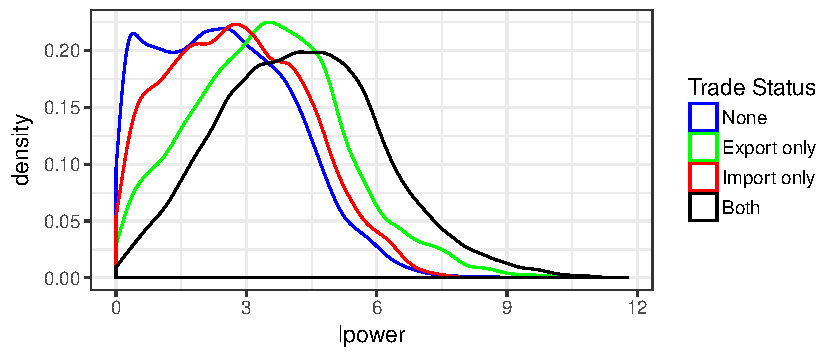
\includegraphics{./PICS/denslpower.pdf}   \\ 
 \input{./TABLES/sumstatslpower.gen}  \\  
\end{tabular}
\end{table}
\end{center}

\subsection{Productivity Estimation (OP,LP,ACF)}\label{prodest}
\subsubsection{\cite{olley1992dynamics} (OP) }\label{op}

 \cite{olley1992dynamics} (OP) use the
following strategy to estimate the Cobb-Douglus function: 


The log transformation of the production function is written as : 
\begin{equation}
y_{it} = \beta_{o} + \beta_{l}l_{it} + \beta_{k}K_{it} + \omega_{it} + \epsilon_{it} 
\end{equation}
where $l_{it}$ is labour, $K_{it}$ is capital, $m_{it}$  is
the demand for materials, $\omega_{it}$ is firm-level-productivity
observable to the firm and $\epsilon_{it}$ are shocks to production.\\
The optimal investment decision of the firm is characterised by the following
function:
\begin{equation}
i_{it}= f_{K}(l_{it-1}, K_{it}, \omega_{it})
\end{equation}
The optimal labor decision is characterised by the following function:
\begin{equation}
l_{it}= f_{K}(l_{it-1}, K_{it}, \omega_{it})
\end{equation}

These are the assumptions made by \textbf{OP}:
\begin{enumerate}
\item $f_{K}(l_{it-1}, K_{it}, \omega_{it})$ is invertible in
  $\omega_{it}$
\item $\omega_{it}$ follows a first order markov process 
\item Investment at period i is not active until period $t+1$:
  $K_{it+1}= (1-\delta)k_{it} + i_{it}$
\item Labor is a perfectly flexible input i.e there are no labor
  adjustment cost
\end{enumerate}

The estimation procedure proceeds in two step:
\begin{enumerate}
\item Estimation of $\beta_{k}$:
Since $\omega_{it}=f_{K}^{-1}(l_{it-1},k_{it},i_{it})$ and inserting
this in the Cobb-Douglus equation to get: 
$$ y_{it} = \beta_{l}l_{it} + \phi_{it}(l_{it-1},i_{it},K_{it})$$
where $\phi_{it}(l_{it-1},i_{it},K_{it}) =  \beta_{k}K_{it}+ f_{K}^{-1}(l_{it-1},k_{it},i_{it})$
$\phi_{it}(l_{it-1},i_{it},K_{it})$ is approximated using a polynomial
expression and $beta_{l}$ is estimated by using OLS on the above
equation
\item Estimation of $\beta_{k}$:
Since $\omega_{it}$ follows a first order markov process, it can be
written as: 
$$ \omega_{it} = h(\omega_{it-1}) + e_{it}$$
Then $\phi_{it}$ can be written as: 
$$ \phi_{it} = beta_{k}K_{it} + h(\omega_{it-1}) + e_{it}$$
$$ \phi_{it} = beta_{k}K_{it} + h(\phi_{it-1}- \beta_{k}k_{it-1}) + e_{it}$$
The unknown form of function h is approximated by quadratic function
and for any value of $\beta_K$ to get:
$$ \hat{\phi_{it}} = beta_{k}K_{it} +\gamma_{0}
\gamma_{1}\hat{\omega_{it-1}^{\beta_{k}}}+
\gamma_{2}(\hat{\omega_{it-1}^{\beta_{k}}})^{2}
+ \gamma_{3}(\hat{\omega_{it-1}^{\beta_{k}}})^{3} $$
 This expression is minimised to get the estimate of $\beta_{k}$. 
\end{enumerate}
\subsubsection{\cite{levinsohn2003estimating} (LP)}
\cite{levinsohn2003estimating} \textbf{LP} uses a similar strategy but use intermediate input demand
as the function to invert out $\omega_{it}$. 
Here, the intermediated material demand function is given by:
$$  m_{it} = m_{it}(\omega_{it}, k_{it})$$
This function is assumed to be montonically increasing and therefore
productivity can be found by inverting the function above. Therefore,
we can write the equation above as: 
$$ y_{it} = \beta_{l}l_{it} + \phi_{it}(m_{it},K_{it})$$
where $\phi_{it}(m_{it},K_{it}) =  \beta_{k}K_{it}+ \omega_{it}(m_{it}, K_{it})$

They suggest to use a third degree polynomial approximation of
$\phi_{it}$ and substitute it into the equation above to give the
following result: 

$$  y_{it} =  \beta_{l}l_{it} + \sum_{i=0}^{3} \sum_{j=0}^{3-i}
\delta_{ij}k_{it}^{i}m_{it}^{j}$$
The coefficient is $\beta_{l}$ is estimtated by OLS using the equation
above and $\hat{\phi_{it}}$ is estimtated by subtracting labor from
the fitted value of the above equation:
$$ \hat{\phi_{it}} = \hat{y_{it}} - \hat{\beta_{l}}l_{it} =
 \sum_{i=0}^{3} \sum_{j=0}^{3-i}
\hat{\delta_{ij}}k_{it}^{i}m_{it}^{j}$$
Therefore, 

So, for any value of $\beta_{k}^{*}$:
$$\hat{\omega_{it}} = \hat{\phi_{it}} - \beta_{k}^{*}k_{it}$$
$$ y_{it}^{*} = y_{it} - \beta_{l}l_{it} = \beta_{k}K_{it}
+ \omega_{it}(m_{it}, K_{it})$$
 
Since it is also assumed that $\omega_{it}$ follows a first order markov
process : 
$$\omega_{it} = E[\omega_{it}|\omega_{it-1}] + \epsilon_{it}$$
They also assume a polynomial expansion of the expectation above to give:
$$ \omega_{it}=  \gamma_{o}+\gamma_{1}\omega_{it-1} +
\gamma_{2}\omega_{it-1}^2 + \gamma_{3}\omega_{it-1}^3 + \epsilon_{it} $$ 

Therefore, the value of $\beta_{K}$, for which the expression below is
minimized is chosen to be the coefficient.  
\begin{equation}
\min_{\beta_{k}^{*}}\sum (y_{it} - \hat{\beta_{l}l_{it}} -
\beta_{k}^{*}K_{it} - \hat{E[\omega_{it}|\omega_{it-1}]})^2 
\end{equation}

\subsubsection{\cite{ackerberg2006structural}(ACF)}
\cite{ackerberg2006structural}(ACF) suggest that labour might be
correlated with productivity and might not be a fully flexible
method and therefore the firms input material demand is written as: 
$$ m_{it} = f_{it}(\omega_{it}, k_{it}, l_{it})$$
Inverting this function for $\omega_{it}$ and substituting into the
production function results in the following 
equation of the form:
\begin{equation}
y_{it} = \beta_{l}l_{it} + \beta_k k_{it} + f_{it}^{-1}(m_{it},
k_{it}, l_{it})+ \epsilon_{it}
\end{equation}
They suggest that the  labor coefficient should be estimated
in the second stage of the estimation since it is correlated with
productivity. 
They suggest the following steps:

\begin{enumerate}
\item Obtain $\phi_{it}(m_{it}, k_{it}, l_{it}) = \beta_{l}l_{it} + \beta_k k_{it} + f_{it}^{-1}(m_{it},
k_{it}, l_{it})$ by regression $y_{it}$ on polynomial approximation of
$\phi_{it}(m_{it}, k_{it}, l_{it})$
\item Use the markovian nature of $\omega_{it} =
  E(\omega_{it}|\omega_{it-1}) + e_{it}$
and use the following moment equations to estimate $\beta_{K}$ and
$\beta_{l}$:
\begin{equation}
E[e_{it}|(k_{it}, l_{it-1})]= 0
\end{equation}
\end{enumerate} 

\input{./TABLES/regLPcont.gen}
\input{./TABLES/prodcont.gen} 

\subsection{Dynamic Biprobit  Model}
Let i be the unit and t be the time. A dynamic random effects probit
is written as: 
$$ y_{it}^{*} = \gamma y_{i,t-1} + x_{it}'\beta + \alpha_{i} +
\epsilon_{it}; y_{it}=1[y_{it}^{*} > 0]$$
where $\gamma$ is the state dependence parameter.

There are three ways to estimate the above equation: 
\begin{enumerate}
\item Treat $y_{i1}$ as exogenously given and do not explain it
\item Heckman Method
\item Wooldridge Method
\end{enumerate} 
Code for bivariate probit model 
\textit{biprobit dumexp dumrd x lnk lagexp lagdumrd year92-year93, r}

\subsection{Self Selection and sunk cost hypothesis}
The self-selection hypothesis states that entry into the trade market
involves fixed and sunk costs and only the most productive firms can
overcome these trade costs. Therefore, to participate in the
export/import market a firm must pay a certain costs and only the most
productive are able to pay the costs. To check this hypothesis, I
estimate a dynamic random effects probit model similar to model used
in \cite{roberts1997decision}. 

They define $Y_{it}$ as the discrete decision to export and use the
following Bellman equation for the firm:
\begin{equation}
V_{it}(S_{it})= max_{Y_{it}}E_{t}(\sum_{j=t}^{\infty} \delta^{t-j}R_{ij}|S_{it})
\end{equation}
 where $\delta$ is the one-period discount factor, $S_{it}$ is the
 relevant state variables affecting the firms decision, $R_{ij}$ is
 the revenue. The equation above can also be written as:
\begin{equation}
V_{it}(S_{it})= max_{Y_{it}}E_{t}(\pi^{D} + Y_{it}(\pi^{X}- f^{X} -
c^{X}(1-Y_{it-1}))  + \sum_{j=t+1}^{\infty} \delta^{t-j}R_{ij}|S_{it})
\end{equation}
 Thus, a firm will participate in the export market if:
\begin{equation}
\pi_{it}^{*} = \pi^{D}+\pi^{D}+ Y_{it}  +
\delta^{t}E_{t}(V_{i,t+1}(S_{it+1}|S_{it},Y_{it}=1) -
V_{i,t+1}(S_{it+1}|S_{it},Y_{it}=1) ) -  (f^{X} + c^{X}(1-Y_{it-1}))
\end{equation}
And the reduced form expression of the equation above becomes: 
\begin{equation}
  d_{it}^{X}=\begin{cases}
   1 , & \text{if $\pi_{it}^{*}>  $}.\\
   0 , & \text{if $\pi_{it}^{*}<  0$}.
  \end{cases}
\end{equation}
To make it a probit model, I write the equation above as a linear
function of firm-level characteristics along with dummy variables for
industry and time. 
\begin{equation}
  d_{it}^{X}=\begin{cases}
   1 , & \text{if $\gamma_{1}^{X} d_{it-1}^{X} + 
\gamma_{3}^{X} \hat{\omega}_{it-1}  + \beta_{1}^{X}K_{it-1}  +
IndustrialDummy_{i}^{X} + TimeDummy_{t}^{X}  + \alpha_{i}+ \epsilon_{it}^{X}>= 0   $}.\\
   0 , & \text{otherwise}.
  \end{cases}
\end{equation}
So if the coefficient of  $d_{it-1}^{X}$ is above. This provides
evidence of sunk cost to participate in the export market and if the
coefficient of $\omega_{t-1}$ is positive, then firms with high
productivity self-select into participation in the export market.

A similar model can be estimated with the discrete decision to import,
since importing also involves additional fixed and sunk costs, a firm
would be only participate in the import market if gets productivity
benefits to overcome the costs. Learning-from-importing has been
demonstrated in the previous section, therefore a firm will import if:
\begin{equation}
\begin{equation}
\pi^  +
\delta^{t}E_{t}(V_{i,t+1}(S_{it+1}|S_{it},d_{it}^{M}=1) -
V_{i,t+1}(S_{it+1}|S_{it},d_{it}^{X}=0) ) -  (f^{M} + c^{M}(1-d_{it-1}^{M}))
\end{equation}
Since $S_{it}$ contains productivity which will benefit from
participating in the import market, a firm will import if the
productivtiy benfits outweigh the costs to participate in the import
market. This can be tested with a reduced form probit model similar to
the discrete decision to export: 
\begin{equation}
  d_{it}^{M}=\begin{cases}
   1 , & \text{if $\gamma_{1}^{X} d_{it-1}^{M} + 
\gamma_{3}^{M} \hat{\omega}_{it-1}  + \beta_{1}^{M}K_{it-1}  +\beta_{2}^{M}L_{it-1}
IndustrialDummy_{i}^{M} + TimeDummy_{t}^{M}  + \alpha_{i}+\epsilon_{it}^{M}>= 0   $}.\\
   0 , & \text{otherwise}.
  \end{cases}
\end{equation}
Therefore, the reduced form equations for both the discrete choices
can be written as:
\begin{equation}
d_{it}^{M} = \gamma_{1}^{M} d_{it-1}^{M} + 
\gamma_{3}^{M} \hat{\omega}_{it-1}  + \beta_{1}^{M}K_{it-1}  +\beta_{2}^{M}L_{it-1}
IndustrialDummy_{i}^{M} + TimeDummy_{t}^{M}  + \alpha_{i}+\epsilon_{it}^{M}
\end{equation}
\begin{equation}
d_{it}^{X} = \gamma_{1}^{X} d_{it-1}^{X} + 
\gamma_{3}^{X} \hat{\omega}_{it-1}  + \beta_{1}^{X}K_{it-1}  +\beta_{2}^{X}L_{it-1}
IndustrialDummy_{i}^{X} + TimeDummy_{t}^{X}  + \alpha_{i}+\epsilon_{it}^{X}
\end{equation}
I use the dynamic random effects probit specification with Wooldridge
method which treats the intial conditions problem by accounting for
the correlation of the initial value with $\alpha$:
$$  \alpha_{i}= \gamma d_{i1}+ \tilde{\alpha_{I}} $$

\end{document}
